\documentclass[a4paper,12pt]{report}
\usepackage[pdftex]{graphicx}
\DeclareGraphicsExtensions{.pdf}
\usepackage{amsmath}
\usepackage{amssymb}

% Title Page
\title{Implementation of Exchange-Correlation Energy (for meta-GGA) in Abinit within the norm-conserving approach}
\author{Aur\'{e}lien Lherbier}


\begin{document}
\maketitle

\begin{abstract}
The aim of this report is first to explain briefly the general procedure for calculation of exchange-correlation energy in Abinit (in case of LDA, GGA) and then to discuss the way the meta-GGA case is treated. This report could be useful to any new developers in Abinit who would like to implement in the subdirectory \texttt{/56\_xc}. In this report I will essentially describe the main structures of some routines such as \texttt{rhohxc.F90}, \texttt{xcden.F90}, \texttt{xcmult.F90} and \texttt{xcpot.F90}.
\end{abstract}



\chapter{Rule of notations}

A rule of notations (see below or at the beginning of \texttt{rhohxc.F90}, at the end of the list of \textit{Local variables}) was proposed in version 6.5.0. In one hand, the idea is to try to keep a certain consistency with the labelling of variables. Indeed the latter have been added little by little by different developers who have their own personal notations. In a second hand, the use of a good labelling of variables facilitate the understanding when reading for the first time the code. In that sence, it is often preferable to give a variable name that sticks the much as possible to the physical quantity to which it corresponds.\\
The following rule of notations is only a proposal which can be off course use or not, depending on you. It can also be modified or be improved.
Here below is the proposition:\\

\begin{itemize}
 \item \texttt{rho} ($\rho$) is the electronic density
 \item \texttt{tau} ($\tau$) is the kinetic energy density
 \item \texttt{exc} ($\varepsilon_{xc}$) is the exchange-correlation energy density per particule
 \item \texttt{epsxc} ($\epsilon_{xc}$) is the exchange-correlation energy density ($\epsilon_{xc}=\rho\times\varepsilon_{xc}$)
 \item \texttt{vxc} ($v_{xc}$) is the exchange-correlation potential
 \item \texttt{bigexc} ($E_{xc}$) is the exchange-correlation energy (for the moment it is still named "\texttt{enxc}")
 \item \texttt{m\_norm} ($\vert m \vert$) is the norm of magnetization\\\\

 \item \texttt{g...} means the gradient ($\nabla$) of something (e.g. : \texttt{grho} means gradient of the electronic density)
 \item \texttt{g...2} means square norm of gradient ($\vert \nabla \vert^2$) of something (e.g. : \texttt{grho2}  means square norm of gradient of the electronic density)
 \item \texttt{l...} means Laplacian ($\Delta \equiv \nabla^2$) of something (e.g. : \texttt{lrho} means Laplacian of electronic density)
 \item \texttt{d...d...} means first derivative of something with regards to something else ($\frac{\partial}{\partial}$).
 \item \texttt{d2...d...d...} means second derivative of \texttt{...} with regards to \texttt{...} and to \texttt{...} ($\frac{\partial^2}{\partial\,\,\partial}$)
 \item etc...
 \item \texttt{d...} without the occurence of the second "\texttt{d}" means that this is an array which regroups several derivatives of the same quantity (e.g. : \texttt{depsxc} can contain $\frac{\partial \epsilon_{xc}}{\partial \rho}$ but also $\frac{\partial \epsilon_{xc}}{\partial \vert \nabla \rho\vert}\cdotp \frac{1}{\vert \nabla \rho\vert}$)\\\\

 \item \texttt{...\_b} means a block of the quantity \texttt{...} ( this is use in mpi loops which treat the data block by block)
 \item \texttt{...\_updn} means that spin up and spin down are available in that array such as data\_updn(..,1) and data\_updn(..,2). (if \texttt{nspden} $\geq2$ off course, otherwise if \texttt{nspden}$=1$ data\_up(..,1) contains the total quantity).
 \item \texttt{...\_apn} in case of positrons are concerned.\\

to be the closest as possible with the libxc notations we also use the following variable names:
 \item \texttt{vxcrho} is the first derivative of the exchange-correlation energy density with regards to the electronic density ($\frac{\partial \epsilon_{xc}}{\partial \rho}\equiv$ \texttt{depsxcdrho} ).
 \item \texttt{vxcgrho} is the first derivative of the exchange-correlation energy density with regards to the gradient of the electronic density ($\frac{\partial \epsilon_{xc}}{\vert \nabla \rho\vert}\equiv$ \texttt{depsxcdgrho}).
 \item \texttt{vxclrho} is the first derivative of the exchange-correlation energy density with regards to the Laplacian of the electronic density ($\frac{\partial \epsilon_{xc}}{\partial \Delta \rho}\equiv$ \texttt{depsxcdlrho}).
 \item \texttt{vxctau} is the first derivative of the exchange-correlation energy density with regards to the kinetic energy density ($\frac{\partial \epsilon_{xc}}{\partial \tau}\equiv$ \texttt{depsxcdtau}).
\end{itemize}

\chapter{Brief remind of exchange correlation equations}

Let first recall the general form of the exchange-correlation energy in the case of meta-GGA. For the moment, we will consider a easier case which is a meta-GGA functional which would not depend on the kinetic energy density ($\tau$). Nevertheless, this latter case still encompasses the LDA and GGA cases.

\begin{equation}
E_{xc}^{MGGA} = \int \epsilon_{xc} \left[ \rho_{\sigma}(\mathbf{r}), \nabla \rho_{\sigma}(\mathbf{r}), \Delta \rho_{\sigma}(\mathbf{r}) \right] d\mathbf{r}
\end{equation}

with $\sigma$ the spin index (up or down). The corresponding exchange-correlation potential is given by

\begin{equation}
v_{xc}^{\sigma} = \frac{\delta E_{xc}^{MGGA}}{\delta \rho_{\sigma}} = \frac{\partial \epsilon_{xc}}{\partial \rho_{\sigma}} - \left( \sum_{\alpha=x,y,z} \nabla_{\alpha} \left( \frac{\partial \epsilon_{xc}}{\partial \nabla_{\alpha} \rho_{\sigma}} \right)  \right) + \Delta \left( \frac{\partial \epsilon_{xc}}{\partial \Delta \rho_{\sigma}} \right) \label{eqvxc}
\end{equation}

The total exchange-correlation energy ($E_{xc}$) is a simple scalar since it is the integral over the whole space ($\int d\mathbf{r}$) of a functional of density (plus eventually its gradient and its Laplacian) which itself depends on the space position ($\mathbf{r}$). On the contrary the potential $v_{xc}$ is a function of the space position ($\mathbf{r}$) and then is a scalar field. In the above equation (Eq.\ref{eqvxc}), the first term on the right hand side is the LDA contribution, the second term is the GGA contribution and the third term is the meta-GGA contribution.
Note that in the code, the second term is not directly expressed in this way but with another form which is

\begin{equation}
\sum_{\alpha=x,y,z} \nabla_{\alpha} \left( \frac{\partial \epsilon_{xc}}{\partial \nabla_{\alpha} \rho_{\sigma}} \right) = \sum_{\alpha=x,y,z} \nabla_{\alpha} \left[ \nabla_{\alpha} \rho_{\sigma} \times \left( \frac{1}{\vert \nabla \rho_{\sigma} \vert }\cdotp \frac{\partial \epsilon_{xc}}{\partial \vert \nabla \rho_{\sigma}\vert } \right) \right]
\end{equation}

with $\vert \nabla \rho_{\sigma} \vert = \left(\sum_{\alpha=x,y,z} \nabla_{\alpha}\rho_{\sigma}\right)^{1/2}$.\\

TO BE COMPLETED FOR THE CASE WHERE KINETIC ENERGY DENSITY IS INVOLVED

\chapter{The routines structures of rhohxc.F90, xcden.F90, xcmult.F90 and xcpot.F90}

\begin{figure}[!ht]
	\centering
	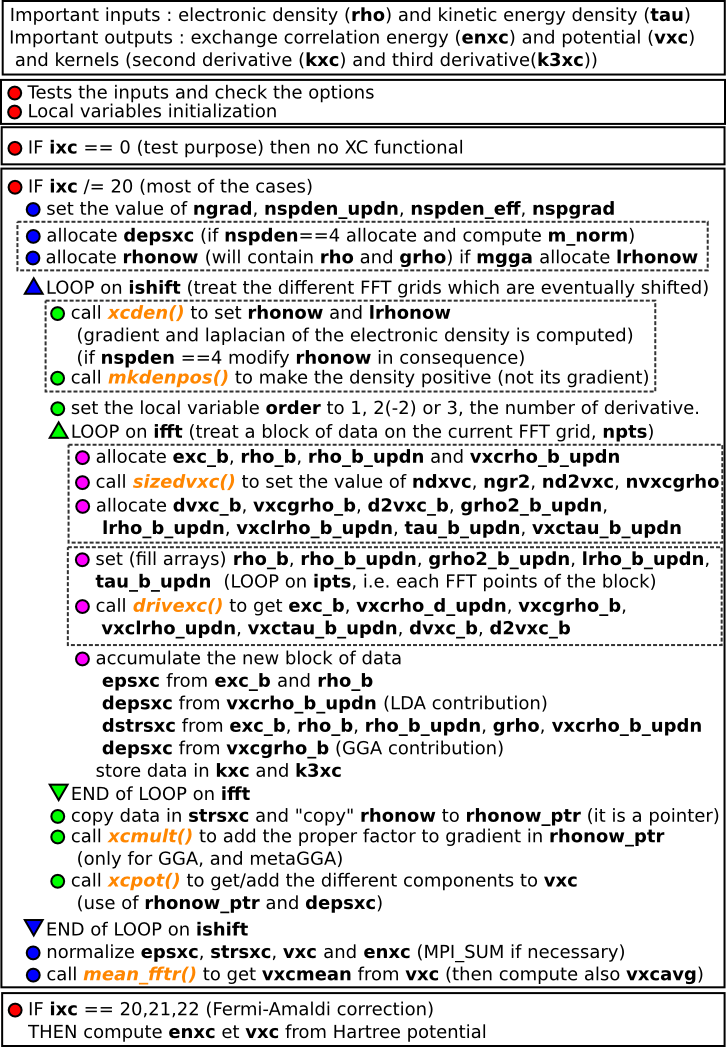
\includegraphics[width=\textwidth]{rhohxc}
	\caption{Scheme of the routine \texttt{rhohxc.F90}.}
	\label{figrhohxc}
\end{figure}

\begin{figure}[!ht]
	\centering
	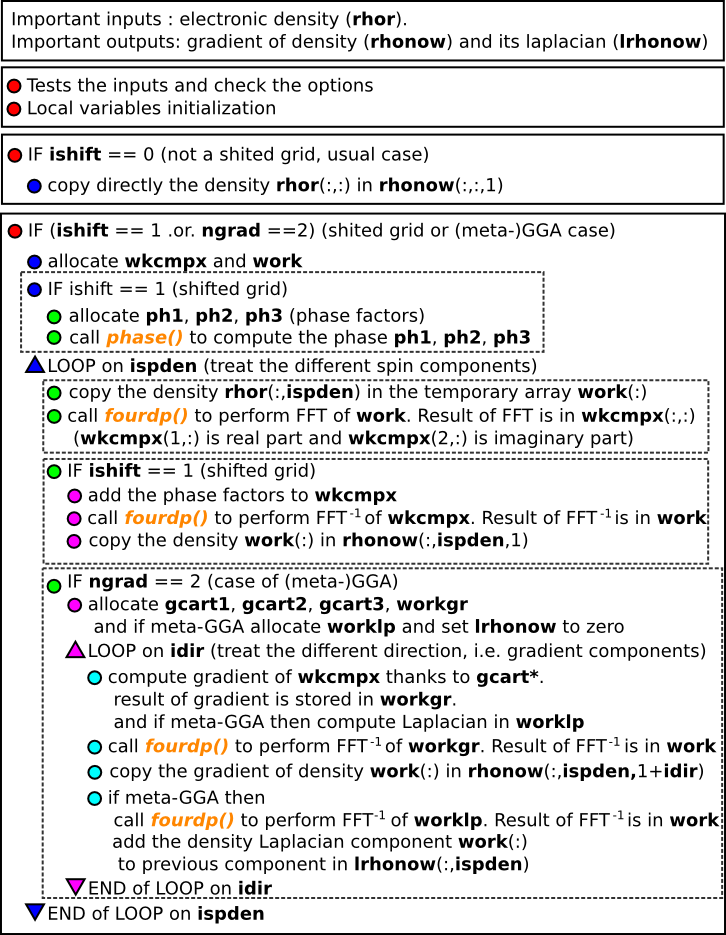
\includegraphics[width=\textwidth]{xcden}
	\caption{Scheme of the routine \texttt{xcden.F90}.}
	\label{figxcden}
\end{figure}

\begin{figure}[!ht]
	\centering
	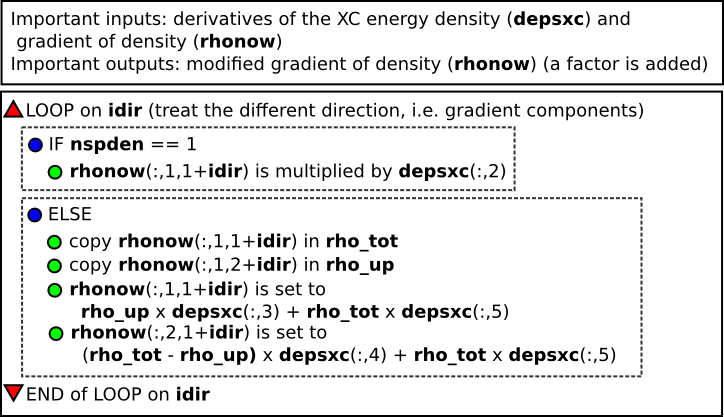
\includegraphics[width=\textwidth]{xcmult}
	\caption{Scheme of the routine \texttt{xcmult.F90}.}
	\label{figxcmult}
\end{figure}

\begin{figure}[!ht]
	\centering
	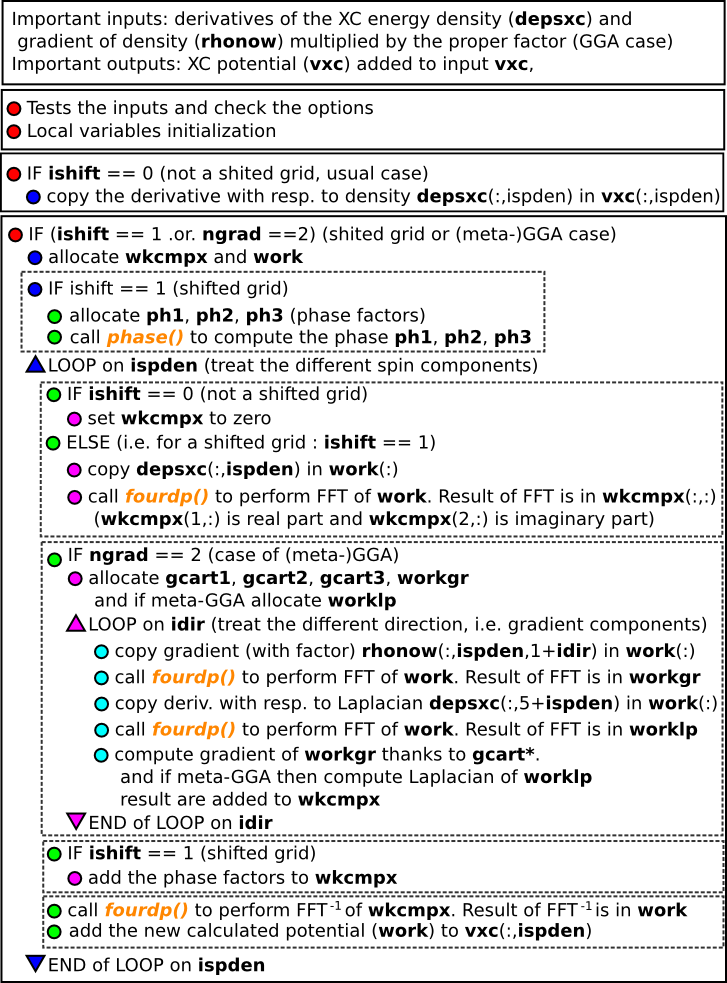
\includegraphics[width=\textwidth]{xcpot}
	\caption{Scheme of the routine \texttt{xcpot.F90}.}
	\label{figxcpot}
\end{figure}

\end{document}
